\begin{remark}
    Soit $P$ un ensemble de propositions. Une formule $\Phi$ de la logique propositionnelle sur $P$ est satisfaisable s'il exite une interprétation
    \begin{equation*}
        V : X \rightarrow \{1, 0\}, \text{telle que } V \models \Phi
    \end{equation*}
\end{remark}
\subsection{Littéraux et Clauses}
\begin{definition}{Littéral}{litteral}
    Un \textbf{littéral} est une variable $x$ ou sa négation $\neg x$.
\end{definition}
\begin{definition}{Clause}{clause}
    Une \textbf{clause} est une disjonction de littéraux $l_1 \vee l_2 \vee \dots \vee l_n$. Elle est satisfaite par une valuation $V$ s'il existe $i$ tel que $V(l_i) = 1$. Par extension, on appelle .
\end{definition}
\begin{example}
    $p$ et $\neg p$ sont des littéraux. $x \vee\neg y \vee r$ est une clause mais pas $x \wedge y$.
\end{example}
\begin{theorem}{Satisfaction d'ensemble de clauses}{satensembleclauses}
    Un ensemble de clauses $A = \{C_1, \dots, C_n\}$ est satisfait par une valuation $V$, notée $V \models A$, si pour tout $i$, $V \models C_i$. En particulier, tout valuation satisfait l'ensemble vide $A = \emptyset$.
\end{theorem}
\subsubsection{Lien avec les formes normales}
\begin{itemize}[label=\textbullet]
    \item Une formule est en forme normale conjonctive (\textbf{FNC}) si et seulement si c'est une conjonction de disjonctions de littéraux, de la forme :
    \begin{equation*}
        \bigwedge_i(\bigvee_j(\neg)x_{i,j})
    \end{equation*}
    \item Une formule est en forme normale disjonctive (\textbf{FND}) si et seulement si c'est une disjonction de conjonctions de littéraux, de la forme :
    \begin{equation*}
        \bigvee_i(\bigwedge_j(\neg)x_{i,j})
    \end{equation*}
\end{itemize}
\begin{lemma}{Equivalence formule FNC}{equiFNC}
    Tout ensemble non-vide de clauses $A = \{C_1,\dots,C_n\}$ est équivalent à la formule en FNC $\Phi_A = \bigwedge_{i=1}^{n} C_i$, au sens où pour toute valuation, $V \models A \Leftrightarrow V \models \Phi_A$.
\end{lemma}
\begin{remark}
    Pour mettre une formule sous forme de clauses, il suffit de la mettre en FNC.
\end{remark}
\subsubsection{Mise sous FNC et FND}\label{sec:mettreFNCFND}
Afin de parvenir à une FNC ou une FND, on utilise les transformations successives suivantes pour obtenir les formes normales :
\begin{enumerate}
    \item élimination des connecteurs $\rightarrow$ et $\leftrightarrow$ grâce aux équivalences suivantes :
    \begin{equation*}
        (\Phi\rightarrow\Psi)\equiv(\neg\Phi\vee\Psi)
    \end{equation*}
    \begin{equation*}
        (\Phi\leftrightarrow\Psi)\equiv(\neg\Psi\vee\Psi)\wedge(\Phi\vee\neg\Psi)
    \end{equation*}
    \item entrer les négations le plus à l'intérieur possible :
    \begin{equation*}
        \neg(\Phi\wedge\Psi)\equiv(\neg\Phi\vee\neg\Psi) \qquad \neg\neg\Phi \equiv \Psi
    \end{equation*}
    \begin{equation*}
        \neg(\Psi\vee\Psi)\equiv(\neg\Phi\wedge\Psi)
    \end{equation*}
    \item utilisation des distributivité de $\vee$ et $\wedge$ :
    \begin{equation*}
        (\Phi\vee(\Psi\wedge\chi )) \equiv (\Phi\vee\Psi)\wedge(\Phi\vee\chi)\text{(mise sous FNC)}
    \end{equation*}
    \begin{equation*}
        (\Phi\wedge(\Psi\vee\chi)) \equiv (\Phi\wedge\Psi)\vee(\Phi\wedge\chi)\text{(mise sous FND)}
    \end{equation*}
\end{enumerate}
\begin{example}
    Illustrons cela à travers un exemple, mettons la formule $\neg(x\leftrightarrow(y\rightarrow r))$
    \begin{enumerate}
        \item on retire les équivalences et implications :
        \begin{equation*}
            \neg((\neg x\vee\neg y \vee r)\wedge(\neg(\neg y\vee r)\vee x))
        \end{equation*}
        \item on pousse les négations à l'intérieur :
        \begin{equation*}
            (x\wedge y\wedge\neg r) \vee ((\neg y\vee r)\wedge\neg x)
        \end{equation*}
        \item on distribue : 
        \begin{equation*}
            (x\wedge y\wedge\neg r)\vee((\neg y\vee r)\wedge\neg x)
        \end{equation*}
        \item et encore : 
        \begin{equation*}
            (x\vee\neg y\vee r)\wedge(y\vee\neg y\vee r)\wedge(\neg r\vee\neg y\vee r)\wedge(x\vee\neg x)\wedge(y\vee\neg x)\wedge(\neg r\vee\neg x)
        \end{equation*}
        \item on retire les formules équivalentes à $\top$ :
        \begin{equation*}
            (x\vee\neg y\vee r)\wedge(y\vee\neg x)\wedge(\neg r\vee\neg x)
        \end{equation*}
    \end{enumerate}
    Invitation à prendre le temps de faire cette démonstrations sur une feuille étape par étape pour voir si tout a bine été compris.
\end{example}

\subsection{Problème SAT}
\begin{definition}{Problème SAT}{problemeSAT}
    Une \textbf{entrée} est un ensemble de clauses $S$. \\
    Une \textbf{sortie} est de la forme : Est-ce que $S$ est \textbf{sat}isfaisable?
\end{definition}
Si $S$ est satisfaisable, on aimerait que l'algorithme nous retourne une valuation $V$ qui satisfait $S$.
\begin{remark}
    Actuellement, on ne sait toujours pas s'il existe un algorithme pour ce problème dont la complexité en temps est polynomiale. L'intuition veut que ce ne soit pas le cas mais aucune preuve n'a pu être fournie jusqu'à présent. Si on parvenait à le prouver, on pourrait gagner un prix d'un million de dollars ;). C'est un problème qui appartient à la classe NP. (cf. chapitre sur la complexité) 
\end{remark}

\subsection{Introduction aux solveurs SAT}
\begin{definition}{Solveur SAT}{solveurSAT}
    Un solveur est un programme qui décidé le problème SAT. Si la formule est satisfaisable, une interprétation qui la satifsait est retournée. Ils ont une complexité au pire cas exponentielle. 
\end{definition}

\subsubsection{Notations pour les grandes disjonctions et conjonctions}
\begin{definition}{disjonction et conjonction}{disjonctionconjonction}
    \begin{itemize}[label=\textbullet]
        \item On appelera \textit{disjonction} une formule de la forme $\Phi_1\vee\Phi_2\vee\dots\vee\Phi_n$ où $n \geq 1$. Attention, lorsque $n=1$, la disjonction est réduite à la seule forme $\Phi_1$. On utilisera l'abbréviation suivante :
        \begin{equation*}
            \bigvee_{i=1}^{n}\Phi_i
        \end{equation*}
        \item On appelera \textit{conjonction} une formule de la forme $\Phi_1\wedge\Phi_2\wedge\dots\wedge\Phi_n$ où $n \geq 1$. Attention, lorsque $n=1$, la conjonction est réduite à la seule forme $\Phi_1$. On utilisera l'abbréviation suivante :
        \begin{equation*}
            \bigwedge_{i=1}^{n}\Phi_i
        \end{equation*}
    \end{itemize}
    
\end{definition}

\subsection{Modélisation}
Dans cette section, nous feront la modélisation du problème des 8 reines, d'autres exemples sont présents dans le cours mais le raisonnement demeure identique.
\begin{figure}[H]
    \centering
    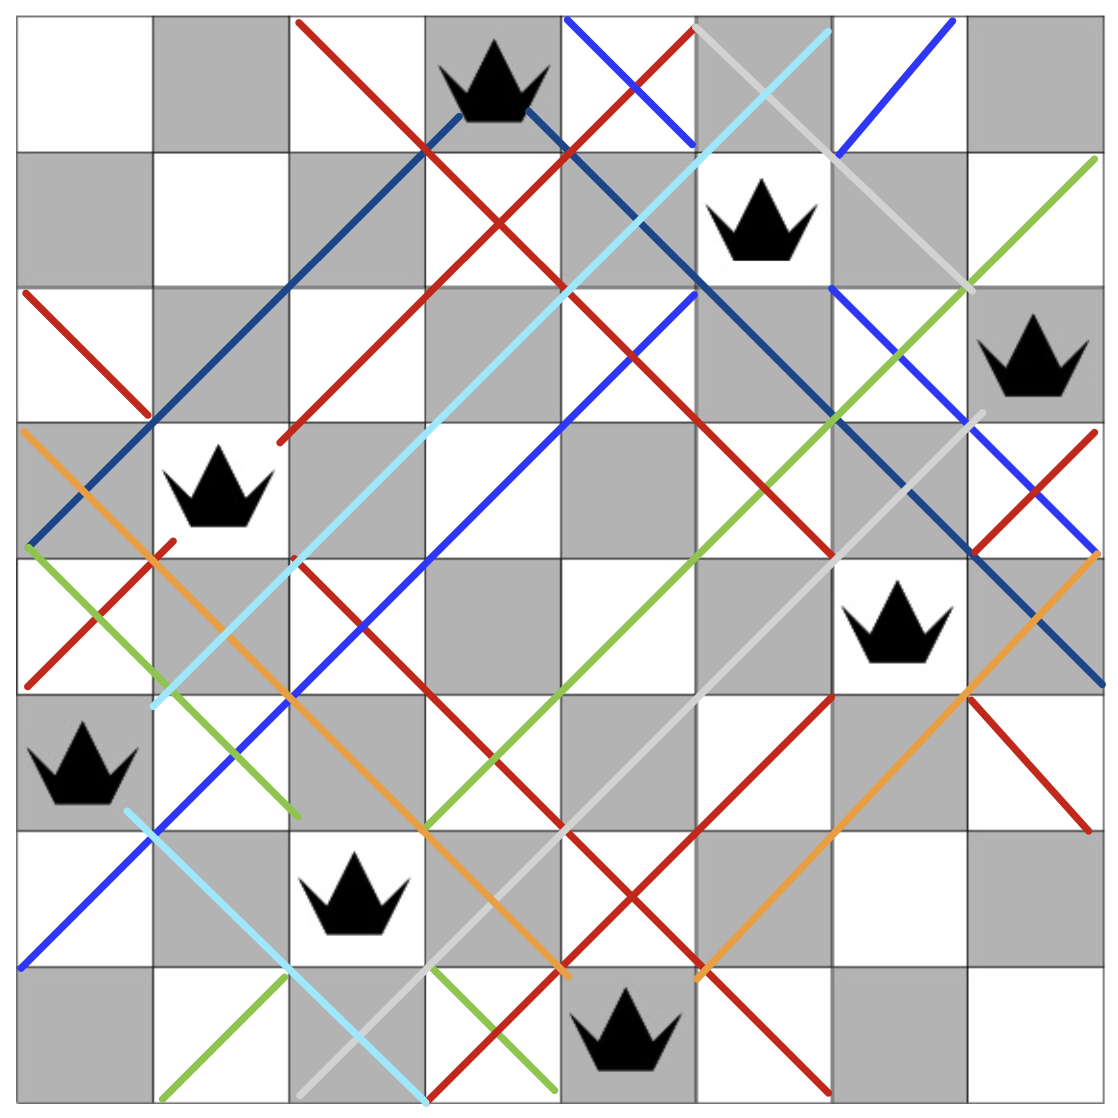
\includegraphics[scale=0.3]{pictures/prob8reines.png}
    \caption{Problème des 8 reines}
    \label{fig:8reines}
\end{figure}
\subsubsection{Choix des variables}
\begin{equation*}
    X = \{x_{i,j} | i,j \in \{1,\dots,8\}\}
\end{equation*}
La sémantique est la suivante : "$x_{i,j}$ est vraie si et seulement s'il y a une reine en case $(i,j)$".

\subsubsection{Expression des contraintes}
\begin{enumerate}
    \item Pas d'attaque horizontale
    \item Pas d'attaque verticale
    \item Pas d'attaque en diagonale
    \item Au moins une reine par ligne
\end{enumerate}

\subsubsection*{Pas d'attaque horizontale}
"Pour toute ligne, il n'existe pas deux reines sur cette ligne."
\begin{equation*}
    \bigwedge_{i \in \{1,\dots,8\}} \neg (\bigvee_{j,j' \in \{1,\dots,8\} | j \neq j'} x_{i,j} \wedge x_{i,k})
\end{equation*}
\begin{equation*}
    \equiv \bigwedge_{i,j,j' \in \{1,\dots,8\} | j \neq j'} (\neg x_{i,j} \vee \neg x_{i,j'})
\end{equation*}
\subsubsection*{Pas d'attaque verticale}
"Pour toute colonne, il n'existe pas deux reines sur cette colonne."
\begin{equation*}
    \bigwedge_{j \in \{1,\dots,8\}} \neg (\bigvee_{i,i' \in \{1,\dots,8\} | i \neq i'} x_{i,j} \wedge x_{k,j})
\end{equation*}
\begin{equation*}
    \equiv \bigwedge_{i,i',j \in \{1,\dots,8\} | i \neq i'} (\neg x_{i,j} \vee \neg x_{i',j})
\end{equation*}
\subsubsection*{Pas d'attaque en diagonale}
"Pour toute diagonale, il n'existe pas deux reines sur cette diagonale."
\begin{equation*}
    \bigwedge_{i,i',j,j' \in \{1,\dots,8\} | i \neq i' \wedge j \neq j'} \neg (x_{i,j} \wedge x_{i',j'} \wedge |i-i'| = |j-j'|)
\end{equation*}
\begin{equation*}
    \equiv \bigwedge_{i,i',j,j' \in \{1,\dots,8\} | i \neq i' \wedge j \neq j'} (\neg x_{i,j} \vee \neg x_{i',j'} \vee |i-i'| \neq |j-j'|)
\end{equation*}
\subsubsection*{Au moins une reine par ligne}
"Pour toute ligne, il existe au moins une reine sur cette ligne."
\begin{equation*}
    \bigwedge_{i \in \{1,\dots,8\}} (\bigvee_{j \in \{1,\dots,8\}} x_{i,j})
\end{equation*}

\subsection{Algorithme DPLL}
Ne sera pas à l'examen.

\subsection{Transformation de Tseitin}
Il se peut que le problème ne s'exprime pas facilement par une formule en FNC. Le but de la transformation de Tseitin est d'ajouter de nouvelles variables et des équivalences.
\begin{example}
    Considérons $\Phi = (x \wedge q) \vee \neg(y \vee r)$, Dans la transformation de Tseitin, on va remplacer $x \wedge q$ par une nouvelle variable $x_1$ et $\neg(y \vee r)$ par une nouvelle variable $x_2$. Voici la formule considérée :
    \begin{equation*}
        (x_1\vee x_2) \wedge (x_1 \leftrightarrow x\wedge q) \wedge (x_2 \leftrightarrow \neg(y\vee r))
    \end{equation*}
    Il reste encore à mattre les deux formules en FNC : (cf. \ref{sec:mettreFNCFND})
    \begin{itemize}[label=\textbullet]
        \item $x_1 \leftrightarrow x \wedge q$
        \begin{equation*}
            \begin{aligned}
                &\equiv (x_1 \rightarrow (x \wedge q)) \wedge ((x \wedge q) \rightarrow x_1) \\
                &\equiv (\neg x_1 \vee (x \wedge q)) \wedge (\neg(x \wedge q) \vee x_1) \\
                &\equiv (\neg x_1 \vee x) \wedge (\neg x_1 \vee q) \wedge (\neg x \vee \neg q \vee x_1)
            \end{aligned}
        \end{equation*}
        \item $x_2 \leftrightarrow \neg(y\vee r)$
        \begin{equation*}
            \begin{aligned}
                &\equiv (x_2 \rightarrow \neg(y\vee r)) \wedge (\neg(y\vee r) \rightarrow x_2) \\
                &\equiv (\neg x_2 \vee \neg y \wedge \neg r)\wedge (y \vee r \vee x_2) \\
                &\equiv (\neg x_2 \vee \neg y) \wedge (\neg x_2 \vee \neg r) \wedge (y \vee r \vee x_2)
            \end{aligned}
        \end{equation*}
    \end{itemize}
    Dès lors, nous pouvons écrire la formule sous FNC suivante :
    \begin{equation*}
        \Psi = (x_1\vee x_2)\wedge(\neg x_1 \vee p)\wedge(\neg x_1\vee q)\wedge(\neg x \vee \neg y \vee x_1)\wedge(\neg x_2 \vee \neg q) \wedge (\neg x_2 \vee \neg r) \wedge (y \vee r \vee x_2)
    \end{equation*}
\end{example}
La transformation de Tseitin est intéressante lorsqu'on devra mettre sous FNC des formules qui sont sous forme normale disjonctive $C_1\vee C_2\vee\dots\vee C_n$. Car il suffit d'introduire une variable $x_i$ pour chaque $C_i$ et on obtient la formule :
\begin{equation*}
    (x_1\vee x_2\vee\dots\vee x_n)\wedge(x_1\leftrightarrow C_1)\wedge\dots\wedge(x_n \leftrightarrow C_n)
\end{equation*} 
Si on suppose que $C_i = l_1\wedge\dots l_k$ où $l_i$ sont des littéraux, alors mettre $x_i\leftrightarrow C_i$ sous FNC est assez simple :
\begin{equation*}
    x_i \leftrightarrow C_i \equiv (\bigwedge_{j=1}^{k}(\neg x_i \vee l_j)) \wedge (x_i \vee \bigvee_{j=1}^{k}(\neg l_j))
\end{equation*}

\warningbox{Il ne faut surtout pas hésiter à ajouter des variables pour minimiser le nombre de clauses.}
